%%%%%%%%%%%%%%%%%%%%%%%%%%%%%%%%% COMMENT THIS TO COMPILE main.tex %%%%%%%%%%%%%%%%%%%%%%%%%%%%%%%%
%\documentclass[a4paper,12pt]{report}
\usepackage[english]{babel}
\usepackage[left=2cm,right=2cm,top=2cm,bottom=2cm]{geometry}
%\usepackage{mathtools}
\usepackage{amsthm}     % for definitions and theorems
\usepackage[many]{tcolorbox}    % boxes around definitions and theorems
%\usepackage{amsmath}
%\usepackage{nccmath}
\usepackage{amssymb}    % \ltimes
\usepackage{etoolbox}   % for start of Chapter
%\usepackage{amsfonts}
\usepackage{physics}    % for all Physics related
\usepackage{dsfont}     % for the identity matrix symbol \1
%\usepackage{mathrsfs}

\usepackage{titling}
\usepackage{indentfirst}

\usepackage{bm}
\usepackage[dvipsnames]{xcolor}
\usepackage{cancel}

\usepackage{xurl}
\usepackage[colorlinks=true]{hyperref}

\usepackage{float}
\usepackage{graphicx}
\usepackage{subcaption}
%\usepackage{tikz}

\usepackage{ctable}     % tabelas
\renewcommand{\P}{\phantom{+}}  % empty space to indent things
\usepackage{multirow}
\usepackage{tabulary}

%%%%%%%%%%%%%%%%%%%%%%%%%%%%%%%%%%%%%%%%%%%%%%%%%%%

\newcommand{\eps}{\epsilon}
\newcommand{\vphi}{\varphi}
\newcommand{\cte}{\text{cte}}

\newcommand{\N}{{\mathbb{N}}}
\newcommand{\Z}{{\mathbb{Z}}}
%\newcommand{\Q}{{\mathbb{Q}}}
\newcommand{\C}{{\mathbb{C}}}
\renewcommand{\S}{{\hat{S}}}
%\renewcommand{\H}{\s{H}}

\renewcommand{\a}{{\vb{a}}}
\renewcommand{\b}{{\vb{b}}}
\renewcommand{\d}{{\dagger}}
\newcommand{\up}{{\uparrow}}
\newcommand{\down}{{\downarrow}}
\newcommand{\hc}{{\text{h.c.}}}

\newcommand{\ihat}{\bm{\hat{\imath}}}
\newcommand{\jhat}{\bm{\hat{\jmath}}}
\newcommand{\khat}{\bm{\hat{k}}}

\newcommand{\0}{{\vb{0}}}
\newcommand{\1}{\mathds{1}}
\newcommand{\E}{{\vb{E}}}
\newcommand{\B}{{\vb{B}}}
\renewcommand{\u}{{\vb{u}}}
\renewcommand{\v}{{\vb{v}}}
\renewcommand{\r}{{\vb{r}}}
\newcommand{\R}{{\vb{R}}}
\newcommand{\Q}{{\vb{Q}}}
\newcommand{\G}{{\vb{G}}}
\newcommand{\g}{{\vb{g}}}
\renewcommand{\k}{{\vb{k}}}
\newcommand{\K}{{\vb{K}}}
\newcommand{\p}{{\vb{p}}}
\newcommand{\q}{{\vb{q}}}
\newcommand{\F}{{\vb{F}}}
\renewcommand{\t}{{\vb{t}}}
\newcommand{\vtau}{{\bm{\tau}}}
\newcommand{\vdelta}{{\bm{\delta}}}

% COLORED SYMMETRY ELEMENTS
\newcommand{\Ct}{{\textcolor{Cyan}{C_3}}}
\newcommand{\Ctn}[1]{{\textcolor{Cyan}{C_3^{\textcolor{black}{#1}}}}}
\newcommand{\Cs}{{\textcolor{ForestGreen}{C_6}}}
\newcommand{\Csn}[1]{{\textcolor{ForestGreen}{C_6^{\textcolor{black}{#1}}}}}
\newcommand{\sd}{{\textcolor{RoyalBlue}{\sigma_d}}}
\newcommand{\sdn}[1]{{\textcolor{RoyalBlue}{\sigma_d^{\textcolor{black}{#1}}}}}
\newcommand{\sdp}{{\textcolor{RoyalBlue}{\sigma_d'}}}
\newcommand{\sdpp}{{\textcolor{RoyalBlue}{\sigma_d''}}}
\newcommand{\sv}{{\textcolor{Orange}{\sigma_v}}}
\newcommand{\svn}[1]{{\textcolor{Orange}{\sigma_v^{\textcolor{black}{#1}}}}}
\newcommand{\svp}{{\textcolor{Orange}{\sigma_v'}}}
\newcommand{\svpp}{{\textcolor{Orange}{\sigma_v''}}}

\newcommand{\s}{\sigma}
%\newcommand{\prodint}[2]{\left\langle #1 , #2 \right\rangle}
\newcommand{\cc}[1]{\overline{#1}}
\newcommand{\Eval}[3]{\eval{\left( #1 \right)}_{#2}^{#3}}
\newcommand{\sg}[2]{\{ #1 \mid #2 \}}

\newcommand{\unit}[1]{\; \mathrm{#1}}

\newcommand{\n}{\medskip}
\newcommand{\e}{\quad \mathrm{and} \quad}
\newcommand{\ou}{\quad \mathrm{or} \quad}
\newcommand{\virg}{\, , \;}
\newcommand{\ptodo}{\forall \,}
\renewcommand{\implies}{\; \Rightarrow \;}
%\newcommand{\eqname}[1]{\tag*{#1}} % Tag equation with name

\setlength{\droptitle}{-7em}

\makeatletter
\patchcmd{\chapter}{\if@openright\cleardoublepage\else\clearpage\fi}{}{}{}  % start 'Chapter' at the same page. needs package etoolbox
\makeatother

%% Theorems, definitions, proofs
\theoremstyle{definition}

\newtheorem{definition}{Definition}[section]
\tcolorboxenvironment{definition}{
  colback=blue!5!white,
  boxrule=0pt,
  boxsep=1pt,
  left=2pt,right=2pt,top=2pt,bottom=2pt,
  oversize=2pt,
  sharp corners,
  before skip=\topsep,
  after skip=\topsep,
}

\newtheorem{theorem}{Theorem}[section]
\tcolorboxenvironment{theorem}{
  colback=blue!5!white,
  boxrule=0pt,
  boxsep=1pt,
  left=2pt,right=2pt,top=2pt,bottom=2pt,
  oversize=2pt,
  sharp corners,
  before skip=\topsep,
  after skip=\topsep,
}

%\begin{document}
%%%%%%%%%%%%%%%%%%%%%%%%%%%%%%%%% COMMENT THIS TO COMPILE main.tex %%%%%%%%%%%%%%%%%%%%%%%%%%%%%%%%


%%%%%%%%%%%%%%%%%%%%%%%%%%%%%%%%%%%%%%%%%%%%%%%%%%%%%%%%%%%%%%%%%%%%%%%%%%%%%%%%%%%%%%%%%%%%%%%%%%
\chapter{Emmergent symmetries and Wannier obstruction in TBG} \label{ch:emmergent_symm_wannier_obstruction}
%%%%%%%%%%%%%%%%%%%%%%%%%%%%%%%%%%%%%%%%%%%%%%%%%%%%%%%%%%%%%%%%%%%%%%%%%%%%%%%%%%%%%%%%%%%%%%%%%%

\textbf{THE TEXT BELOW IS PLACEHOLDER. IT WAS COPIED FROM PREVIOUS REPORTS}

Regarding (a), in Section \ref{sec:tbg}, we present our progress in understanding the MATBG system by studying its geometry \cite{handbook2019}, the Bistritzer-MacDonald (BM) model \cite{macdonald2011}, and its symmetry properties \cite{thesis_rennella}. Symmetry analysis is a prerequisite for comprehending the Wannier obstruction phenomenon \cite{zou2018}, which arises from the non-trivial topology of the electronic bands. This phenomenon refers to the impossibility of representing the flat bands using exponentially localized Wannier functions that preserve all symmetries of the band structure. In contrast, the THF model addresses this issue by providing a fully symmetric framework that reformulates and maps the interacting MATBG as a topological heavy fermion system \cite{topoheavyfermion2022}.

We initiated our exploration of the MATBG theory with reference to \cite{handbook2019}, aiming primarily to comprehend the Moiré pattern geometry and the Bistritzer-MacDonald continuous model \cite{macdonald2011}. Subsequently, our focus shifted to analyzing the system's symmetries \cite{thesis_rennella}, which are pivotal, with implications such as the Wannier obstruction \cite{zou2018}. In Section \ref{sec:tbg}, we elucidate our studies.

By implementing the BM model \cite{macdonald2011}, when we twist the two graphene layers (from the initial AB stacking) by a discrete set of very specific angles, with the first being $\theta \approx 1.05^\circ$, the bands should become very flat around the point $K$, which corresponds to the low-energy excitations of the system.

\textbf{THE TEXT ABOVE IS PLACEHOLDER. IT WAS COPIED FROM PREVIOUS REPORTS}

%%%%%%%%%%%%%%%%%%%%%%%%%%%%%%%%%%%%%%%%%%%%%%%%%%%%%%%%%%%%%%%%%%%%%%%%%%%%%%%%%%%%%%%%%%%%%%%%%%
\section{Commensurate structures} \label{sec:tbg_geom}
%%%%%%%%%%%%%%%%%%%%%%%%%%%%%%%%%%%%%%%%%%%%%%%%%%%%%%%%%%%%%%%%%%%%%%%%%%%%%%%%%%%%%%%%%%%%%%%%%%

Twisted bilayer graphene (TBG) features two graphene layers rotated relative to each other by an angle \( \theta \). This rotation gives rise to a Moiré pattern, formed by the interference of the two lattices. The pattern can be either \textit{commensurate}, exhibiting translational symmetry and forming a periodic superlattice, or \textit{incommensurate}, lacking translational symmetry and periodicity. Figure \ref{fig:moireD6} illustrates a commensurate Moiré pattern with \( D_6 \) point group symmetry, where the rotation center lies at the center of a hexagon. The AA, AB, and BA regions in the pattern represent areas where \( A \) or \( B \) carbon atoms from the layers align with each other.

The system can generally exhibit different symmetry groups depending on the choice of the origin for the rotation by \( \theta \). However, the largest possible point group is \( D_6 \), due to the honeycomb Bravais lattice of the two layers. In the commensurate case, the primitive lattice vectors \( \vb{L}_1 \) and \( \vb{L}_2 \) are defined as the least common multiples of the unit vectors of the monolayers. Figure \ref{fig:latvec} provides an example for \( \theta = 21.8^\circ \).
\begin{figure}[H]
\centering
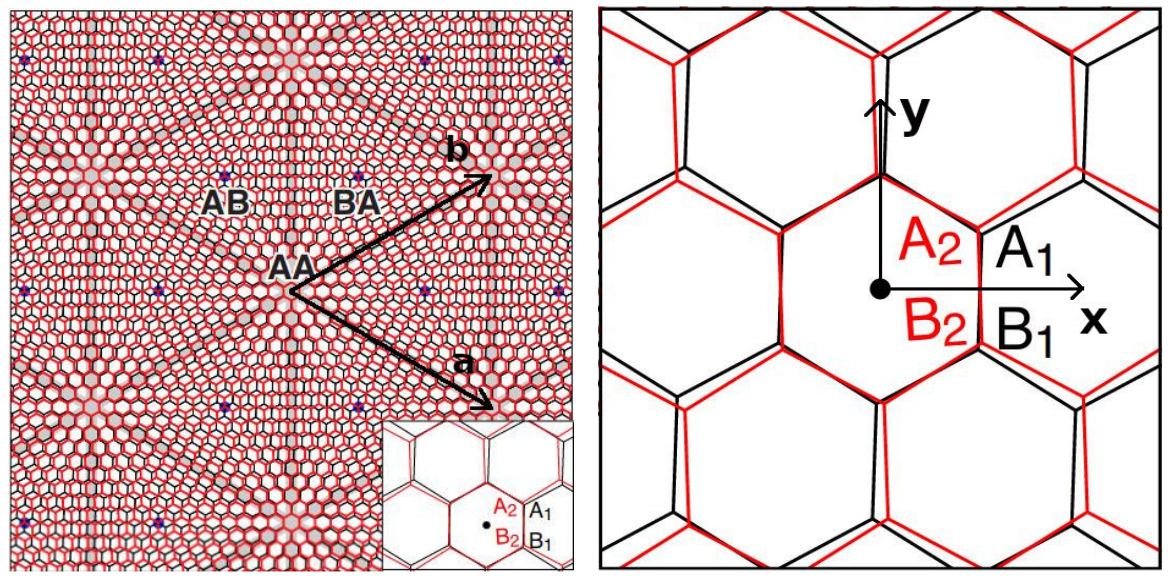
\includegraphics[height=.32\columnwidth]{fig/moireD6.png}
\caption{Commensurate $D_6$-type structure obtained by twisting the two layers from the initial AA stacking configuration, with the origin chosen as the center of the hexagons. Figure taken from \cite{thesis_rennella}.}
\label{fig:moireD6}
\end{figure}

%As drawn in Figure \ref{fig:latvec}, we have
%\begin{align}
%\label{eq:scalarprods1}
%\vb{a}_1^{(1)} \vdot \vb{a}_2^{(1)} &= a^2 \cos(60^\circ) = a^2/2; \\
%\label{eq:scalarprods2}
%\vb{a}_1^{(1)} \vdot \vb{a}_1^{(2)} &= a^2 \cos\theta; \\
%\label{eq:scalarprods3}
%\vb{a}_1^{(1)} \vdot \vb{a}_2^{(2)} &= a^2 \cos(60^\circ + \theta); \\
%\label{eq:scalarprods4}
%\vb{a}_1^{(2)} \vdot \vb{a}_2^{(1)} &= a^2 \cos(60^\circ - \theta).
%\end{align}

The superlattice vectors $\vb{L}_1$, $\vb{L}_2$ are related by a $60^\circ$ rotation. In general, because $\vb{L}_1$ belongs to the lattices of both layers, it can be parameterized by integers $n_1^{(1)}, n_2^{(1)}, n_1^{(2)}, n_2^{(2)}$ as
\begin{equation} \label{eq:L1}
\vb{L}_1 = n_1^{(1)}\vb{a}_1^{(1)} + n_2^{(1)}\vb{a}_2^{(1)} = n_1^{(2)}\vb{a}_1^{(2)} + n_2^{(2)}\vb{a}_2^{(2)},
\end{equation}
where $\vb{a}_{1,2}^{(\ell)}$ are the unit vectors of layer $\ell = 1,2$.

The resulting crystal will exhibit exact lattice translational symmetry with the superlattice vectors \( \vb{L}_1 \) and \( \vb{L}_2 \) only if \( \theta \) satisfies the commensurability condition \cite{thesis_rennella, zou2018}, given by integers \( m \) and \( r \):

\begin{equation} \label{eq:costheta}
\cos\theta(m,r) = \frac{3m^2 + 3mr + r^2/2}{3m^2 + 3mr + r^2} = \frac{3 + 3 \qty(\frac{r}{m}) + \frac{1}{2} \qty(\frac{r}{m})^2}{3 + 3 \qty(\frac{r}{m}) + \qty(\frac{r}{m})^2}.
\end{equation}

We point out that \( \theta(m,r) \) is a function of only the ratio \( r/m \) and is monotonic within the range \( 0 \leq \theta \leq 60^\circ \). Therefore, all commensurate angles can be uniquely determined by pairs of coprime integers \( (m, r) \), where \( \gcd(m, r) = 1 \).

There are two types of structures, classified as Type I and Type II \cite{zou2018} (or SE-odd and SE-even, respectively, with SE standing for sublattice exchange \cite{continuum_model_lopesdossantos2012}), each characterized by distinct relationships between the superlattice vectors \(\vb{L}_1\) and \(\vb{L}_2\) and the primitive vectors of the layers. These relationships can be expressed in terms of the primitive vectors of the first layer, \(\a_1^{(1)}\) and \(\a_2^{(1)}\), as follows:
\begin{itemize}

\item \textit{Type I (SE-odd)}, when $\gcd(r, 3) = 1$:
\begin{equation} \label{eq:type-I-L1L2}
\begin{pmatrix}
\vb{L}_1 \\ \vb{L}_2
\end{pmatrix} =
%\begin{pmatrix}
%1 & -1 \\
%1 & 0
%\end{pmatrix}
%\begin{pmatrix}
%m & 2m+r \\
%-(m+r) & m
%\end{pmatrix}
%\begin{pmatrix}
%1 & 0 \\
%-1 & 1
%\end{pmatrix}
%\begin{pmatrix}
%\a_1^* \\ \a_2^*
%\end{pmatrix}
%=
\begin{pmatrix}
m & m+r \\
-(m+r) & 2m+r
\end{pmatrix}
\begin{pmatrix}
\a_1^{(1)} \\ \a_2^{(2)}
\end{pmatrix}.
\end{equation}

\item \textit{Type II (SE-even)} when $\gcd(r,3) = 3$:

\begin{equation} \label{eq:type-II-L1L2}
\begin{pmatrix}
\vb{L}_1 \\ \vb{L}_2
\end{pmatrix} =
%\begin{pmatrix}
%1 & -1 \\
%1 & 0
%\end{pmatrix}
%\begin{pmatrix}
%m+\frac{r}{3} & m+\frac{2r}{3} \\
%-\frac{r}{3} & m+\frac{r}{3}
%\end{pmatrix}
%\begin{pmatrix}
%1 & 0 \\
%-1 & 1
%\end{pmatrix}
%\begin{pmatrix}
%\a_1^{*} \\ \a_2^{*}
%\end{pmatrix}
%=
\begin{pmatrix}
m+\frac{r}{3} & \frac{r}{3} \\
-\frac{r}{3} & m+\frac{2r}{3}
\end{pmatrix}
\begin{pmatrix}
\a_1^{(1)} \\ \a_2^{(2)}
\end{pmatrix}.
\end{equation}

\end{itemize}

For both Type I and Type II structures, the moiré lattice constant \( L(m, r) = \abs{\vb{L}_1} = \abs{\vb{L}_2} \) is determined by the following formula:
\begin{equation} \label{eq:commensurate-constant}
L(m, r) = a \sqrt{\frac{3m^2 + 3mr + r^2}{\gcd(r, 3)}},
\end{equation}
where \(a = 0.246 \unit{nm}\) is the lattice constant of the monolayer, and \(\gcd(r, 3)\) accounts for the sublattice exchange parity.

The area of the unit cell of the moiré superlattice is given by
\begin{equation} \label{eq:superlattice_area_unitcell}
A_{\text{moiré}} = \frac{\sqrt{3}}{2} L^2 = \frac{3m^2 + 3mr + r^2}{\gcd(r,3)} \, A_1,
\end{equation}
where \( A_1 = \frac{\sqrt{3}}{2} \, a^2 \) represents the area of the unit cell of monolayer graphene. As the unit cell area of the moiré superlattice increases, its corresponding Brillouin Zone shrinks, forming what is referred to as the mini Brillouin Zone (mBZ). The area of the mBZ is given by
\begin{equation} \label{eq:bz-volume}
\Omega_{\text{mBZ}} = \frac{(2\pi)^2}{A_{\text{moiré}}} = \frac{\gcd(r,3)}{3m^2 + 3mr + r^2} \, \Omega_1,
\end{equation}
where \( \Omega_1 = \frac{(2\pi)^2}{A_1} \) is the area of the monolayer's BZ.

For instance, when \( (m, r) = (1, 1) \), we have \( \gcd(r,3) = 1 \) (Type I structure) and a corresponding twist angle \( \theta(1,1) = 21.8^\circ \). In this case, \( 3m^2 + 3mr + r^2 = 7 \), meaning that the monolayer BZ accommodates 7 mBZs within its area, as illustrated in Figure \ref{fig:bzminibz}.

\begin{figure}[H]
\centering
\begin{subfigure}{.5\textwidth}
  \centering
  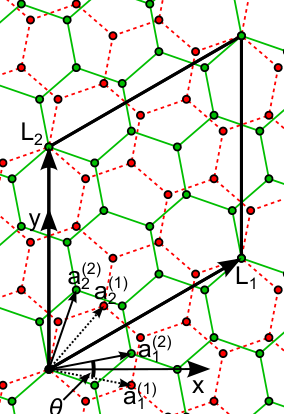
\includegraphics[height=.6\linewidth]{fig/latvec.png}
  \caption{}
  \label{fig:latvec}
\end{subfigure}%
\begin{subfigure}{.5\textwidth}
  \centering
  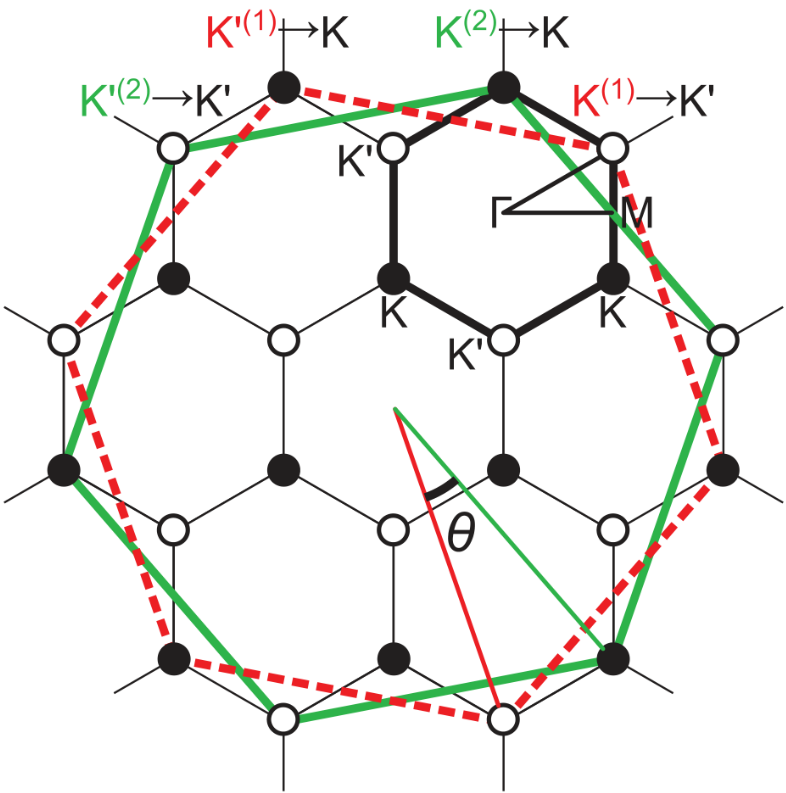
\includegraphics[height=.6\linewidth]{fig/bzminibz.png}
  \caption{}
  \label{fig:bzminibz}
\end{subfigure}
\caption{(a) Commensurate structure and lattice vectors $\vb{L}_1$, $\vb{L}_2$. (b) Monolayers (red and green) and mini BZ's with $(m,r) = (1,1)$ and $\theta = 21.8^\circ$. Figures taken from \cite{koshino2012}. \textbf{SEPARAR AS FIGURAS}}
\label{fig:geometry}
\end{figure}

The distinct relationships between the superlattice vectors for Type I and Type II structures lead to different folding patterns for the Dirac points \(K^{(1)}\) and \(K^{(2)}\) of the monolayers into the mBZ. In Type I structures, the Dirac points \(K^{(1)}\) and \(K^{(2)}\) fold into different time-reversal types of Dirac points in the mBZ, with \(K^{(1)}\) folding to \(K_m'\) and \(K^{(2)}\) folding to \(K_m\), as illustrated in Figure \ref{fig:bzminibz}. In contrast, for Type II structures, \(K^{(1)}\) and \(K^{(2)}\) fold into the same type of Dirac point, \(K_m\), in the mBZ. For a more detailed discussion of these folding patterns, refer to \cite{zou2018}.


We emphasize that the commensuration condition for TBG depends only on the twist angle $\theta$, not the twisting center. As long as the twist angle satisfies Equation \ref{eq:costheta}, the bilayer retains exact translational symmetry, even if the twisting center is a generic point where no two carbon atoms align perfectly. The Moiré lattice vectors $\vb{L}_1$ and $\vb{L}_2$, lattice constant \( L(m, r) \), and momentum mapping between the microscopic and Moiré Brillouin zones (BZs) depend solely on the twist angle and not the twisting center. However, the twisting center determines the exact point-group symmetries of the commensurate lattice. If the twisting center is a generic point, translations are the only exact spatial symmetries. If it is the center of a hexagon as in Figure \ref{fig:moireD6}, the twisted bilayer graphene (TBG) inherits the six-fold rotational symmetry \( C_6 \) of the monolayers.

\pagebreak

From the discussion above, one would conclude that a commensurate TBG system should have a translational symmetry with lattice constant $L(\theta)$ given by Eq. \eqref{eq:commensurate-constant}. However, as discussed in \cite{zou2018}, scanning tunneling microscopy (STM) experiments actually observe an effective moiré lattice constant
\begin{equation} \label{eq:STM-constant}
L'(\theta) = \frac{a}{2 \sin(\theta/2)} \leq \frac{r}{\sqrt{\gcd(r,3)}} \cdot \frac{a}{2 \sin(\theta/2)} = L(\theta).
\end{equation}

This can be interpreted as TBG exhibiting an approximate translational symmetry with superlattice constant $L'(\theta)$, despite optionally possessing an exact translational symmetry with $L(\theta)$ in the commensurate case.

The Bistritzer-MacDonald model (also known as the ``continuum theory'') incorporates translational symmetry by a lattice constant $L'(\theta)$ and other emergent symmetries observed in TBG experiments. This theory describes the system at every twist angle $\theta \lesssim 10^\circ$, including incommensurate ones \cite{continuum_model_castroneto2007, macdonald2011}. It predicts universal features, such as Dirac crossings between valence and conduction bands in each valley, which match tight-binding calculations for commensurate structures and experimental data for larger twist angles, where correlation effects are less significant \cite{zou2018}. However, the theory underestimates the gap between the nearly flat bands and the other bands. This discrepancy can be addressed by incorporating effects like lattice relaxation and electron interactions, which can be phenomenologically accounted for by adjusting the model's parameters \cite{koshinohubbard2018}.

The continuum theory includes additional symmetries, such as \(C_6 T\) rotation and valley \(U_v(1)\) symmetries, which, while not fully present in commensurate structures, are essential for protecting Dirac points in valley-filtered bands. The \(C_2 T = (C_6 T)^3\) symmetry prevents the Dirac points from opening a gap. Although these symmetries are approximations, they remain effective in small-angle TBG experiments, making the differences between commensurate and incommensurate structures negligible.

A key feature of the band structure is the inability to construct well-localized Wannier functions that respect all symmetry operations. This issue arises because some symmetries in the continuum theory, such as \(C_2 T\) and \(U_v(1)\), are not exact microscopic symmetries, yet they are essential for preserving Dirac crossings.

In conclusion, it is essential to study systems with translational, \(C_6 T\), and \(U_v(1)\) emergent symmetries, even though fully implementing these symmetries leads to a Wannier obstruction in the band structure. In Section \ref{sec:BM-model}, we derive the continuum model, and in Section \ref{sec:wannier_obstruction}, we address the related Wannier obstruction.

%%%%%%%%%%%%%%%%%%%%%%%%%%%%%%%%%%%%%%%%%%%%%%%%%%%%%%%%%%%%%%%%%%%%%%%%%%%%%%%%%%%%%%%%%%%%%%%%%%
\section{Bistritzer-MacDonald model} \label{sec:BM-model}
%%%%%%%%%%%%%%%%%%%%%%%%%%%%%%%%%%%%%%%%%%%%%%%%%%%%%%%%%%%%%%%%%%%%%%%%%%%%%%%%%%%%%%%%%%%%%%%%%%

<++> <++> <++> <++> <++> <++> <++> <++> <++> <++> <++> <++> <++>

The atoms positions of each layer are given by
\begin{equation} \label{eq:position-atoms-tbg}
\r = n_1 \a_{\ell,1} + n_2 \a_{\ell,2} + \vtau_{\ell,\alpha},
\end{equation}
where $\alpha = A,B$ indexes the site type, and $\tau_{\ell,\alpha}$ are basis vectors. The lattice vectors are the rotated $\a_{j}^{(\ell)} = R_{\theta_\ell} \a_{j}$, where
\begin{equation} \label{eq:rotation-matrix}
R_\theta =
\begin{pmatrix}
\cos\theta & -\sin\theta \\
\sin\theta & \cos\theta
\end{pmatrix},
\end{equation}
is the rotation matrix by an angle $\theta$ and we use the reference frame which $\theta_1 = -\theta/2$ and $\theta_2 = +\theta/2$. We shall consider AB-stacking as the starting position ($\theta=0$), because this is the most stable configuration for bilayer graphene \cite{handbook2019}. In this case, the translation vectors are given by
\begin{align}
\tau_{1,A} &= R_{-\theta/2}(0,0), \quad \tau_{2,A} = R_{\theta/2} [(0,-d) + \vtau_0], \label{eq:tauA} \\
\tau_{1,B} &= R_{-\theta/2}(0,d), \quad \tau_{2,B} = R_{\theta/2} [(0,0) + \vtau_0], \label{eq:tauB}
\end{align}
where $\vtau_0$ is an arbitrary translation. For example, $\vtau_0 = (0,0)$ corresponds to AB-stacking and $\vtau_0 = (0, d)$ corresponds to AA-stacking.

Defining the wave vectors $\vb{G}_{\ell,1} = \vb{b}_{\ell,1}$, $\vb{G}_{\ell,2} = \vb{b}_{\ell,2}$ and $\vb{G}_{\ell,3} = \vb{b}_{\ell,1} - \vb{b}_{\ell,2}$, the moiré pattern can be interpreted by an beat effect with periodicity $\vb{b}_k^{\text{m}} = \vb{G}_{1,k} - \vb{G}_{2,k}$, \cite{handbook2019}:
\begin{equation} \label{eq:moire-bvecs}
\vb{b}_1^{\text{m}} = \sqrt{3} \abs{\Delta \K} \qty( \frac{1}{2}, -\frac{\sqrt{3}}{2}), \quad
\vb{b}_2^{\text{m}} = \sqrt{3} \abs{\Delta \K} \qty( \frac{1}{2},  \frac{\sqrt{3}}{2}),
\end{equation}
where $\K$ is a Dirac point of an unrotated monolayer, and $\Delta\K = \K_1-\K_2$ with $\abs{\Delta \K} = 2 \abs{\K} \sin(\theta/2)$.

\n

The Hamiltonian $H$ of the model comes from a tight-binding approach $H = H_1 + H_2 + H_{\perp}$, where $H_\ell$ is the Hamiltonian of the layer $\ell$, and $H_\perp = V_{12} + V_{12}^\d$ describes the interlayer hybridization. We write this Hamiltonian in terms of Bloch waves
\begin{equation} \label{eq:BM-blochwave}
\ket{\psi_{\ell, \k, \alpha}} = \frac{1}{\sqrt{N_\ell}} \sum_{\R_\ell} e^{i \k \vdot (\R_\ell + \vtau_{\ell,\alpha})} \ket{\ell, R_\ell, \alpha},
\end{equation}
where $\ell$ labels the layer, $N_\ell$ is the number of unit cells, $\R_\ell$ are the positions of the underlying Bravais lattice, $\vtau_{\ell,\alpha}$ are the orbital centers (of sublattice $\alpha = A,B$) in the unit cell, and $\ket{\ell,\R_\ell,\alpha}$ are localized Wannier states. In this basis, considering only nearest-neighbor intralayer hopping, the low-energy Hamiltonian of each layer is
\begin{equation} \label{eq:blg-eachlayer-hamil-lowenergy}
H^{\pm \K}(\q) = \hbar v_F \abs{\q}
\begin{pmatrix}
0 & e^{\mp i (\theta_\q - \theta_\ell)} \\
e^{\pm i (\theta_\q - \theta_\ell)} & 0
\end{pmatrix},
\end{equation}
where we expanded $\k = \pm \K_\ell + \q$ to first-order in $\q$.

\n

The interlayer Hamiltonian in second quantization reads
\begin{equation} \label{eq:interlayer-hopping}
V_{12} = \sum_{\R_1,\alpha,\R_2,\beta} c_{1,\alpha}^\d t_{12}^{\alpha\beta}(\R_1,\R_2) c_{2,\beta}(\R_2), \quad
t_{12}^{\alpha\beta}(\R_1,\R_2) =
\mel{1,\R_1,\alpha}{V_{12}}{2,\R_2,\beta}.
\end{equation}

Performing the Fourier transformation
\begin{equation} \label{eq:blg-fourier}
c_{\ell,\alpha}^\d(\R_\ell) = \frac{1}{\sqrt{N_\ell}} \sum_{\k_\ell}
e^{-i\k_\ell \vdot (\R_\ell + \vtau_{\ell,\alpha})} c_{\ell,\alpha}^\d(\k_\ell),
\end{equation}
with the sum of $\k_\ell$ over the BZ of layer $\ell$, we have
\begin{equation} \label{eq:interlayer-hopping-kspace}
V_{12} = \sum_{\k_1,\alpha,\k_2,\beta} c_{1,\alpha}^\d(\k_1) T_{12}^{\alpha\beta}(\k_1,\k_2) c_{2,\beta}(\k_2),
\end{equation}
\begin{equation} \label{eq:interlayer-hopping-Tkspace}
T_{12}^{\alpha\beta}(\k_1,\k_2) =
\frac{1}{\sqrt{N_1 N_2}} \sum_{\R_1,\R_2} e^{-i\k_1\vdot(\R_1+\vtau_{1,\alpha})}
t_{12}^{\alpha\beta}(\R_1,\R_2) e^{i\k_2\vdot(\R_2+\vtau_{2,\beta})}.
\end{equation}

Assuming the interlayer hopping $t_{12}^{\alpha\beta}(\R_1,\R_2)$ is only a function of the separation between the centers of the two orbitals, we can apply a Fourier transformation
\begin{equation} \label{eq:interlayer-hopping-fourier}
t_{12}^{\alpha\beta}(\R_1,\R_2) = t_{12}^{\alpha\beta}(\R_1+\vtau_{1,\alpha}-\R_2-\vtau_{2,\beta}) =
\int \frac{\dd[2]{\p}}{(2\pi)^2} e^{i \p \vdot (\R_1+\vtau_{1,\alpha}-\R_2-\vtau_{2,\beta})} t_{12}^{\alpha\beta}(\p).
\end{equation}

Plugging Eq. \eqref{eq:interlayer-hopping-fourier} in Eq. \eqref{eq:interlayer-hopping-Tkspace}, we obtain
\begin{equation} \label{eq:interlayer-hopping-simplified}
T_{12}^{\alpha\beta}(\k_1,\k_2) = \frac{1}{A_1}
\sum_{\G_1, \G_2} e^{i\G_1\vdot\vtau_{1,\alpha}} t_{12}^{\alpha\beta}(\p)
e^{-i\G_2\vdot\vtau_{2,\beta}} \delta_{\k_1+\G_1, \k_2+\G_2},
\end{equation}
where the crystal momentum coupling $\k_1 + \G_1 = \k_2 + \G_2$ is known as generalized umklapp condition.

\n

Equation \eqref{eq:interlayer-hopping-simplified} relies on the functional form of $t_{12}^{\alpha\beta}(\mathbf{p})$. In order to make further progress, we introduce additional assumptions. Given that both $A$ and $B$ sites of graphene correspond to a $p_z$ orbital of carbon atoms, we assume that $t_{12}^{\alpha\beta}(\r) = t_\perp(\r)$ does not depend on $\alpha$ or $\beta$. In \cite{tperp-laissardiere2012}, the authors characterize the behavior of $t_\perp(\r)$ using Slater-Koster parameters and numerically evaluate $t_\perp(\mathbf{p})$ through Eq. \eqref{eq:interlayer-hopping-fourier}. They establish that $t_\perp(\p)$ is solely a function of $\abs{\p}$ with rapid decay. This has significant implications, as only a few umklapp processes contribute to the coupling in Eq. \eqref{eq:interlayer-hopping-simplified}.

\n

In the small angle limit $\theta \lesssim 10^\circ$, we can expand $\k_\ell = \K_\ell + \q_\ell$ around the Dirac points of each layer, with $\abs{\q_\ell} \sim \abs{\Delta \K} \ll \abs{\K}$. Approximating $t_\perp(\K_1+\q_1+\G_1) \approx t_\perp(\K_1+\G_1)$, the interlayer coupling becomes
\begin{equation} \label{eq:interlayer-hopping-truncation}
T_{12}^{\alpha\beta}(\q_1,\q_2) = \frac{1}{A_{1}} \sum_{\G_1,\G_2} e^{i\G_1\vdot\vtau_{1,\alpha}}
t_{12}^{\alpha\beta}(\K_1+\G_1) e^{-i\G_2\vdot\vtau_{2,\beta}}
\delta_{\K_1+\q_1+\G_1,\K_2+\q_2+\G_2}.
\end{equation}

As $t_\perp(\p)$ rapidly decays with $\abs{\p}$, we truncate $t_\perp(\p) \approx 0$ for $\abs{\p} > \abs{\K}$. This leaves us with only three options for $\G_\ell$, where it can be either $\g_{\ell 1} = 0$, $\g_{\ell 2} = \b_{\ell 2}$, or $\g_{\ell 3} = -\b_{\ell 1}$. These options correspond to the three equivalent Dirac points on the monolayer Brillouin zone. Therefore, the crucial quantity becomes $t\perp(\abs{\K})$. This truncation leaves us with the term
\begin{equation} \label{eq:delta-term}
\delta_{\K_1+\q_1+\G_1,\K_2+\q_2+\G_2} = \delta_{\q_2-\q_1,\K_1-\K_2+\G_1-\G_2}.
\end{equation}

Since $\abs{\q_\ell} \ll \abs{\K}$, we find that the condition $\q_2-\q_1 = \K_1-\K_2+\G_1-\G_2$ is true only when $\G_1 = \g_{1n}$ and $\G_2 = \g_{2n}$ have the same index $n$. Consequently, we encounter three possibilities of momentum transfer:
\begin{equation} \label{eq:qb}
\q_\text{b} = \K_1 - \K_2 = \abs{\Delta \K} \, \qty(0, -1),
\end{equation}
\begin{equation} \label{eq:qtr}
\q_\text{tr} = (\K_1 - \K_2) + (\g_{12} - \g_{22}) = \abs{\Delta \K} \, \qty(\frac{\sqrt{3}}{2}, \frac{1}{2}),
\end{equation}
\begin{equation} \label{eq:qtl}
\q_\text{tl} = (\K_1 - \K_2) + (\g_{13} - \g_{23}) = \abs{\Delta \K} \, \qty(-\frac{\sqrt{3}}{2}, \frac{1}{2}),
\end{equation}

Finally, the interlayer coupling ends up with only three terms
\begin{equation} \label{eq:interlayer-3terms}
T_{12}^{\alpha\beta}(\q_1,\q_2) =
T^{\alpha\beta}_{\q_\text{b}} \delta_{\q_1-\q_2, \q_\text{b}} +
T^{\alpha\beta}_{\q_\text{tr}} \delta_{\q_1-\q_2, -\q_\text{tr}} +
T^{\alpha\beta}_{\q_\text{tl}} \delta_{\q_1-\q_2, -\q_\text{tl}},
\end{equation}
where
\begin{equation} \label{eq:interlayer-tensor}
T^{\alpha\beta}_{\q_n} = \frac{t_\perp(\abs{\K})}{A_{\text{u.c.}}} e^{i \g_{1n} \vdot \bm{\tau}_{1\alpha}}
e^{-i \g_{2n} \vdot \bm{\tau}_{2\beta}}.
\end{equation}

Writing matrices in the $A, B$ basis we get
\begin{equation} \label{eq:T-qb}
T_{\q_\text{b}} = \frac{t_\perp(\abs{\K})}{A_{\text{u.c.}}}
\begin{pmatrix}
1 & 1 \\
1 & 1
\end{pmatrix},
\end{equation}
\begin{equation} \label{eq:T-qtr}
T_{\q_\text{tr}} = \frac{t_\perp(\abs{\K})}{A_{\text{u.c.}}} e^{-i \g_{12} \vdot \vtau_0}
\begin{pmatrix}
e^{i\phi} & 1 \\
e^{-i\phi} & e^{i\phi}
\end{pmatrix},
\end{equation}
\begin{equation} \label{eq:T-qtl}
T_{\q_\text{tl}} = \frac{t_\perp(\abs{\K})}{A_{\text{u.c.}}} e^{-i \g_{13} \vdot \vtau_0}
\begin{pmatrix}
e^{-i\phi} & 1 \\
e^{i\phi} & e^{-i\phi}
\end{pmatrix},
\end{equation}
where $\phi = 2\pi/3$.


%%%%%%%%%%%%%%%%%%%%%%%%%%%%%%%%%%%%%%%%%%%%%%%%%%%%%%%%%%%%%%%%%%%%%%%%%%%%%%%%%%%%%%%%%%%%%%%%%%
\section{Symmetry analysis and Wannier obstruction} \label{sec:wannier_obstruction}
%%%%%%%%%%%%%%%%%%%%%%%%%%%%%%%%%%%%%%%%%%%%%%%%%%%%%%%%%%%%%%%%%%%%%%%%%%%%%%%%%%%%%%%%%%%%%%%%%%

As discussed in \cite{zou2018}, at currently accessible energy scales, experiments indicate that MATBG exhibits some approximate symmetries. These include translational symmetry characterized by the constant $L' = a / (2 \sin\theta/2)$, valley symmetry $U_v(1)$, $C_{2z} \mathcal{T}$, and $D_6$ point group symmetry, which are not fully captured by a generic commensurate structure described in Section \ref{sec:tbg_geom}. The continuum model outlined in Section \ref{sec:BM-model} incorporates all these ``good'' symmetries. In this section, we will explore group theory concepts that will later be applied to understand the Wannier Obstruction \cite{zou2018} and the Topological Heavy Fermion model of MATBG \cite{topoheavyfermion2022}.

For our purposes, the MATBG system exhibits emergent symmetries compatible with the $P622$ space group \cite{thesis_rennella}, which is symmorphic and associated with the $D_6$ point group.

For TBG, we focus on the Wyckoff position $2c$ (\textbf{NO! WE DO NOT!}), corresponding to the AB and BA regions of interest in Figure \ref{fig:moireD6}. The site-symmetry groups of these regions are all isomorphic to the point group $D_3$, a subgroup of $D_6$. In contrast, the $AA$ regions belong to Wyckoff position $1a$, and their site-symmetry groups have higher symmetry $D_6$.

The BM model is advantageous as it is independent of whether a configuration of TBG is commensurate or not, and it also incorporates all the emergent symmetries observed in experiments \cite{zou2018}.

%%%%%%%%%%%%%%%%%%%%%%%%%%%%%%%%%%%%%%%%%%%%%%%%%%%%%%%%%%%%%%%%%%%%%%%%%%%%%%%%%%%%%%%%%%%%%%%%%%
\section{Monolayer}
%%%%%%%%%%%%%%%%%%%%%%%%%%%%%%%%%%%%%%%%%%%%%%%%%%%%%%%%%%%%%%%%%%%%%%%%%%%%%%%%%%%%%%%%%%%%%%%%%%

Considering only nearest-neighbors, the hamiltonian of a single unrotated layer of graphene is given by
$$
H_{\text{mono}}(\k) = -t
\begin{pmatrix}
0 & f(\k) \\
f^*(\k) & 0
\end{pmatrix}
, \quad \ell = 1, 2,
$$
where $f = \sum_{i=1}^{3} e^{i \k \vdot \bm{\delta}}$, and $\bm{\delta}$ are the three nearest-neighbor vectors from a site $A$ of the honeycomb lattice.

Expanding in first-order $\k = \K + \q$, where $\K = \frac{4\pi}{3a} (1, 0)$ is the Dirac point of the unrotated layer, we have
$$
H_{\text{mono}}(\K + \q) \approx v_F \, \q \vdot \bm{\sigma}.
$$

%%%%%%%%%%%%%%%%%%%%%%%%%%%%%%%%%%%%%%%%%%%%%%%%%%%%%%%%%%%%%%%%%%%%%%%%%%%%%%%%%%%%%%%%%%%%%%%%%%
\section{BM model review}
%%%%%%%%%%%%%%%%%%%%%%%%%%%%%%%%%%%%%%%%%%%%%%%%%%%%%%%%%%%%%%%%%%%%%%%%%%%%%%%%%%%%%%%%%%%%%%%%%%

The hamiltonian of the BM model is given by
$$
H = H_1 + H_2 + V + V^\dagger,
$$
where $H_1$ and $H_2$ correspond to the layers 1 and 2, and $V$ is the hybridization between them.

\n

For this discussion, we use the reference frame where layer 1 is unrotated and layer 2 is rotated counter-clockwise by an angle $\theta$. Therefore, we have
$$
H_1(\k) = H_{\text{mono}}(\k), \quad H_2(\k) = H_1(R_\theta^{-1}\k),
$$
$$
R_\theta =
\begin{pmatrix}
\cos\theta & -\sin\theta \\
\sin\theta & \cos\theta
\end{pmatrix}.
$$

Also, the Dirac points of each layer are
$$
\K_1 = \K = \frac{4\pi}{3a} (1, 0), \quad \K_2 = R_\theta \K_1 = R_\theta \K,
$$
$$
$$

Therefore, expanding around the Dirac points $\K_1$ and $\K_2$, respectively:
$$
H_1(\K_1 + \q) \approx v_F \, \q \vdot \bm{\sigma}.
$$
$$
\boxed{ H_2(\K_2 + \q) = H_2(R_\theta \K_1 + \q) = H_1(\K_1 + R_\theta^{-1}\q) \approx v_F \, (R_\theta^{-1}\q) \vdot \bm{\sigma} \approx v_F \, (1 - i \theta \sigma_y ) \, \q \vdot \bm{\sigma}. }
$$

If we \textbf{neglect the $\theta$-dependence on $H_2$}, our BM model will be \textbf{particle-hole symmetric}, as defined by Bernevig.

\n

Of course, the more difficult part is due to the hybridization term $V$. It is written on the Bloch basis $\ket{\ell, \alpha, \p}$, where $\ell = 1, 2$ is the layer index, $\alpha = A, B$ is the sublattice index, and $\p$ is the momentum.
We have
$$
V_{\alpha\beta}(\p, \p') = \bra{1, \alpha, \p} H \ket{2, \beta, \p'}.
$$

When we expand both $\p = \K_1 + \q$ and $\p' = \K_2 + \q'$, \textbf{after the BM considerations}, we get
$$
V_{\alpha\beta}(\K + \q, R_\theta \K + \q') \approx
w \sum_{j=1}^{3} \delta_{\q, \q' + \q_j} T_{\alpha\beta}^j,
$$
where $\q_1, \q_2, \q_3$ are the moiré momentum vectors, with absolute value $k_D = 2 \sin(\theta/2) \abs{\K}$. The matrices $T^j_{\alpha\beta}$ are
$$
T_1 = \sigma_0 + \sigma_x
$$
$$
T_2 = \sigma_0 + \cos(\frac{2\pi}{3}) \sigma_x + \sin(\frac{2\pi}{3}) \sigma_y
$$
$$
T_3 = \sigma_0 + \cos(\frac{2\pi}{3}) \sigma_x - \sin(\frac{2\pi}{3}) \sigma_y
$$
\begin{figure}[H]
\centering
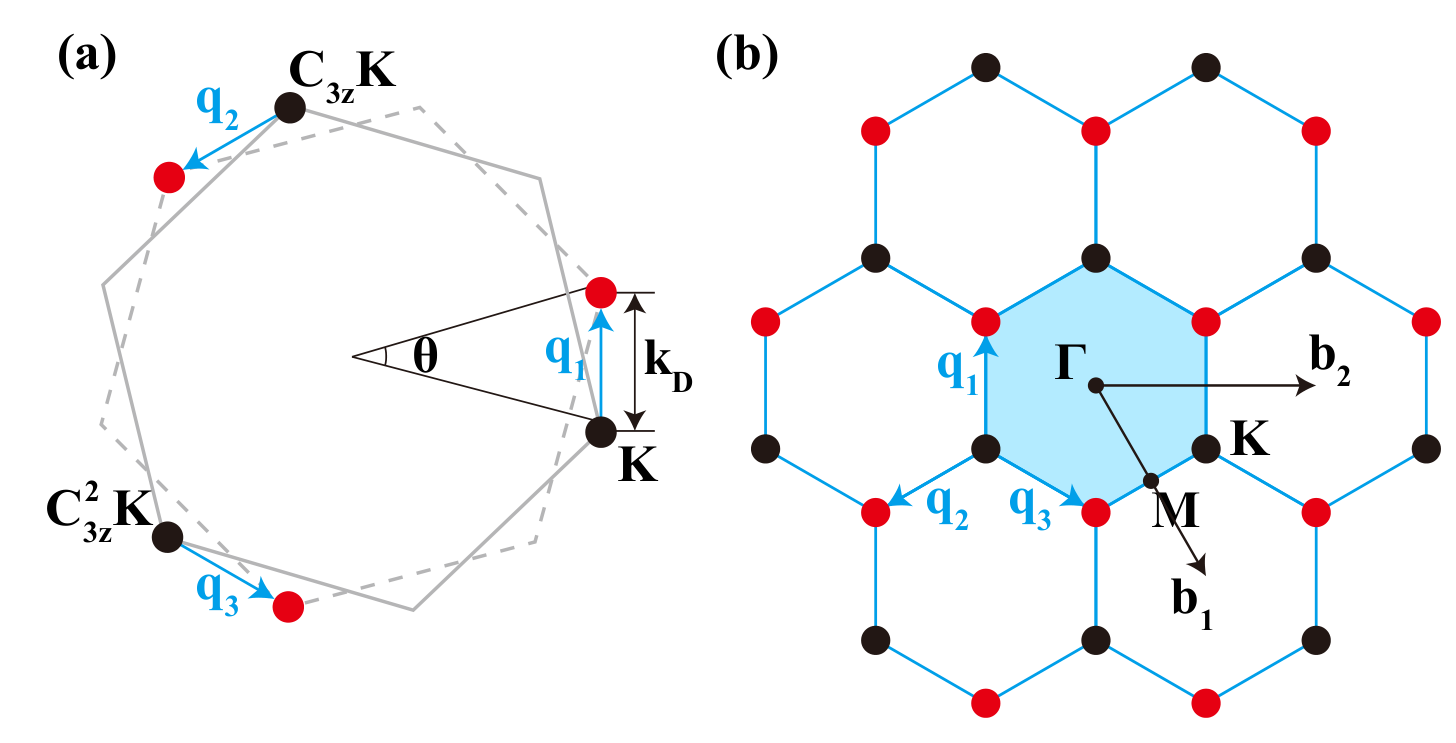
\includegraphics[width=0.8\linewidth]{fig/moire-vectors.png}
\end{figure}

\n

This \textbf{BM model} is called \textbf{MBM-1V (Moiré Band Model - One Valley)} by Bernevig. If we decompose $\q = \k - \Q$, $\q'=\k-\Q'$, where $\Q$ and $\Q'$ belong to the hexagonal lattice formed by adding $\q_{1,2,3}$ iteratively, we can rewrite the hamiltonian as
$$
\boxed{
H_{\Q, \Q'}^{(\text{MBM-1V})}(\k) =
\delta_{\Q,\Q'} v_F (\k-\Q) \vdot \bm{\sigma}
+ w \sum_{j=1}^{3} (\delta_{\Q'-\Q, \q_j} + \delta_{\Q-\Q', \q_j}) T^j.
}
$$

\begin{itemize}
\item This model is \textbf{topological} and is what we have been discussing the whole time.
\item The tables of Bernevig apply to this model, where we consider the Wyckoff position 1a within the THF approach to solve the topological obstruction.
\item Its magnetic space group is $P6'2'2$. Generators: $C_{6z} T$, $C_{2y} T$, $C_{2x}$.
\end{itemize}

\begin{table}[H]
\scriptsize
\caption{Elementary band representations of the magnetic space group $P6'2'2$.}
\centering
\begin{tabular}{|c|c|c|c|c|c|c|c|c|}
\hline
Wyckoff & \multicolumn{3}{c|}{$1a$} & \multicolumn{3}{c|}{$2c$} & \multicolumn{2}{c|}{$3f$} \\
\cline{1-9}
Site sym. & \multicolumn{3}{c|}{$6'2'2$, $32$} & \multicolumn{3}{c|}{$32$, $32$} & \multicolumn{2}{c|}{$2'2'2$, $2$} \\
\cline{1-9}
EBR & $G_{A_1}^{1a}(1)$ & $G_{A_2}^{1a}(1)$ & $G_{E}^{1a}(2)$ & $G_{A_1}^{2c}(2)$ & $G_{A_2}^{2c}(2)$ & $G_{E}^{2c}(4)$   & $G_{A}^{3f}(3)$ & $G_{B}^{3f}(3)$ \\
\hline
$\Gamma$ & $\Gamma_1(1)$ & $\Gamma_2(1)$ & $\Gamma_3(1)$ & $2\Gamma_1(1)$ & $2\Gamma_2(1)$ & $2\Gamma_3(2)$ & $\Gamma_1(1)+\Gamma_3(2)$ & $\Gamma_2(1)+\Gamma_3(2)$ \\
\hline
$K$ & $K_1(1)$ & $K_1(1)$ & $K_2 K_3(2)$ & $K_2 K_3(2)$ & $K_2 K_3(2)$ & $2K_1(1) + K_2 K_3(2)$ & $K_1(1)+K_2 K_3(2)$ & $K_1(1)+K_2 K_3(2)$ \\
\hline
$M$ & $M_1(1)$ & $M_2(1)$ & $M_1(1)+M_2(1)$ & $2M_1(1)$ & $2M_2(1)$ & $2M_1(1)+2M_2(1)$ & $2M_1(1)+M_2(1)$ & $M_1(1)+2M_2(2)$ \\
\hline
\end{tabular}
\label{tab:ebr-P6'2'2}
\end{table}

\begin{table}[H]
\caption{Character table of irreps at high symmetry momenta in magnetic space group $P6'2'2$.}
\centering
\begin{tabular} { c c c c | c c c | c c c }
\cline{1-10}
$\P$ & $\P \Gamma_1$ & $\P \Gamma_2$ & $\P \Gamma_3$ & $\P$ & $\P M_1$ & $\P M_2$ & $\P$ & $\P K_1$ & $\P K_2K_3$ \\
\cline{1-10}
$E$ & $\P1$ & $\P1$ & $\P2$ & $\P E$ & $\P1$ & $\P1$ & $\P E$ & $\P1$ & $\P2$ \\
$2 C_3$ & $\P1$ & $\P1$ & $ -1$ & $\P C_2'$ & $\P1$ & $ -1$ & $\P C_3$ & $\P1$ & $ -1$ \\
$3 C_2'$ & $\P1$ & $ -1$ & $\P0$ & $\P$ & $\P$ & $\P$ & $\P C_3^{-1}$ & $\P1$ & $-1$ \\
\cline{1-10}
\end{tabular}
\label{tab:char-P6'2'2}
\end{table}

%%%%%%%%%%%%%%%%%%%%%%%%%%%%%%%%%%%%%%%%%%%%%%%%%%%%%%%%%%%%%%%%%%%%%%%%%%%%%%%%%%%%%%%%%%%%%%%%%%
\section{There exists another model}
%%%%%%%%%%%%%%%%%%%%%%%%%%%%%%%%%%%%%%%%%%%%%%%%%%%%%%%%%%%%%%%%%%%%%%%%%%%%%%%%%%%%%%%%%%%%%%%%%%

According to Bernevig: ``The MBM-1V is half of the TBG system, with similar physics taking place in the electron states around $\K'$''. A model with the two valleys can be written as
$$
\boxed{
H_{\Q, \Q'}^{(\text{MBM-2V})}(\k) =
\delta_{\Q,\Q'} v_F (\k-\Q) \vdot \bm{\sigma} \otimes \tau_z
+ w \sum_{j=1}^{3} (\delta_{\Q'-\Q, \q_j} + \delta_{\Q-\Q', \q_j}) T^j \otimes \tau_0.
}
$$

Here $\tau_z$ and $\tau_0$ are the Pauli and identity matrix representing the valley degree of freedom.

\begin{itemize}
\item This model is \textbf{apparently different} from the latter, and \textbf{is not topological}. You can decompose it in EBR's as $G_{A_1}^{2c} + G_{A_2}^{2c}$.
\item The tables of Rennella apply to this model. There the authors (Vafek, Rennella, Angeli, Koshino, etc) consider Wyckoff position 2c, because these positions really correspond to symmetry-adapted exponentially localized Wannier functions.
\item The magnetic space group is $P6221'$. Generators: $C_{6z}$, $C_{2y}$, $C_{2x}$, $T$.
\end{itemize}

\begin{table}[H]
\caption{Elementary band representations generated from Wyckoff position $2c$ of the space group $P622$.}
\centering
\begin{tabular}{|c|c|c|c|}
\hline
Wyckoff & \multicolumn{3}{c|}{$2c$} \\
\cline{1-4}
Site sym. & \multicolumn{3}{c|}{$32$} \\
\cline{1-4}
EBR & $G_{A_1}^{2c}(2)$ & $G_{A_2}^{2c}(2)$ & $G_{E}^{2c}(4)$  \\
\hline
$\Gamma$ & $\Gamma_1(1) + \Gamma_4(1)$ & $\Gamma_2(1) + \Gamma_3(1)$ & $\Gamma_5(2) + \Gamma_6(2)$ \\
\hline
$K$ & $K_3(2)$ & $K_3(2)$ & $K_1(1) + K_2(1) + K_3(2)$ \\
\hline
$M$ & $M_1(1) + M_4(1)$ & $M_2(1) + M_3(1)$ & $M_1(1) + M_2(1) + M_3(1) + M_4(1)$ \\
\hline
\end{tabular}
\label{tab:ebr-P622}
\end{table}

\begin{table}[H]
\caption{Character table of irreps at high symmetry momenta in space group $P622$.}
\scriptsize
\centering
\begin{tabular} { c c c c c c c | c c c c c | c c c c }
\cline{1-16}
$\P$ & $\P \Gamma_1$ & $\P \Gamma_2$ & $\P \Gamma_3$ & $\P \Gamma_4$ & $\P \Gamma_5$ & $\P \Gamma_6$ & $\P$ & $\P M_1$ & $\P M_2$ & $\P M_3$ & $\P M_4$ & $\P$ & $\P K_1$ & $\P K_2$ & $\P K_3$\\
\cline{1-16}
$E$      & $\P1$ & $\P1$ & $\P1$ & $\P1$ & $\P2$ & $\P2$ & $E$     & $\P1$ & $\P1$  & $\P1$ & $\P1$ & $E$      & $\P1$ & $\P1$ & $\P2$ \\
$2C_6$   & $\P1$ & $\P1$ & $ -1$ & $ -1$ & $ -1$ & $\P1$ & $C_2$   & $\P1$ & $\P1$  & $ -1$ & $ -1$ & $C_3$    & $\P1$ & $\P1$ & $ -1$ \\
$2C_3$   & $\P1$ & $\P1$ & $\P1$ & $\P1$ & $ -1$ & $ -1$ & $C_2'$  & $\P1$ & $ -1$  & $ -1$ & $\P1$ & $3C_2''$ & $\P1$ & $ -1$ & $\P0$ \\
$C_2$    & $\P1$ & $\P1$ & $ -1$ & $ -1$ & $\P2$ & $ -2$ & $C_2''$ & $\P1$ & $ -1$  & $\P1$ & $ -1$ &          &       &       &       \\
$3C_2'$  & $\P1$ & $ -1$ & $ -1$ & $\P1$ & $\P0$ & $\P0$ &         &       &        &       &       &          &       &       &       \\
$3C_2''$ & $\P1$ & $ -1$ & $\P1$ & $ -1$ & $\P0$ & $\P0$ &         &       &        &       &       &          &       &       &       \\
\cline{1-16}
\end{tabular}
\label{tab:char-P622}
\end{table}

Compare tables \ref{tab:ebr-P622} and \ref{tab:char-P622} with tables 2.5 and (2.1, 2.3) of Rennella \cite{thesis_rennella}, respectively.


%%%%%%%%%%%%%%%%%%%%%%%%%%%%%%%%%%%%%%%%%%%%%%%%%%%%%%%%%%%%%%%%%%%%%%%%%%%%%%%%%%%%%%%%%%%%%%%%%%
\section{\textcolor{red}{DOWN BELOW INCOMPLETE OLD TEXT}}
%%%%%%%%%%%%%%%%%%%%%%%%%%%%%%%%%%%%%%%%%%%%%%%%%%%%%%%%%%%%%%%%%%%%%%%%%%%%%%%%%%%%%%%%%%%%%%%%%%

%%%%%%%%%%%%%%%%%%%%%%%%%%%%%%%%%%%%%%%%%%%%%%%%%%%%%%%%%%%%%%%%%%%%%%%%%%%%%%%%%%%%%%%%%%%%%%%%%%
\subsection{Bistritzer-MacDonald Model}
%%%%%%%%%%%%%%%%%%%%%%%%%%%%%%%%%%%%%%%%%%%%%%%%%%%%%%%%%%%%%%%%%%%%%%%%%%%%%%%%%%%%%%%%%%%%%%%%%%

%%%%%%%%%%%%%%%%%%%%%%%%%%%%%%%%%%%%%%%%%%%%%%%%%%%%%%%%%%%%%%%%%%%%%%%%%%%%%%%%%%%%%%%%%%%%%%%%%%
\subsection{Geometry}
%%%%%%%%%%%%%%%%%%%%%%%%%%%%%%%%%%%%%%%%%%%%%%%%%%%%%%%%%%%%%%%%%%%%%%%%%%%%%%%%%%%%%%%%%%%%%%%%%%

The atoms positions of the each layer are given by
\begin{equation} \label{eq:position-atoms-tbg}
\r = n_1 \a_{\ell,1} + n_2 \a_{\ell,2} + \vtau_{\ell,\alpha},
\end{equation}
where $\alpha = A,B$ indexes the type of the site, and $\tau_{\ell,\alpha}$ are basis vectors. The lattice vectors of each layer are the rotated $\a_{\ell,j} = R_{\theta_\ell} \a_{j}$, where
\begin{equation} \label{eq:rotation-matrix}
R_\theta =
\begin{pmatrix}
\cos\theta & -\sin\theta \\
\sin\theta & \cos\theta
\end{pmatrix},
\end{equation}
is the rotation matrix by an angle $\theta$ and we use the reference frame where $\theta_1 = -\theta/2$ and $\theta_2 = +\theta/2$.

We shall consider AB-stacking. In this case, the translation vectors are given by
\begin{align}
\tau_{1,A} &= R_{-\theta/2}(0,0), \quad \tau_{2,A} = R_{\theta/2} [(0,-d) + \vtau_0], \label{eq:tauA} \\
\tau_{1,B} &= R_{-\theta/2}(0,d), \quad \tau_{2,B} = R_{\theta/2} [(0,0) + \vtau_0], \label{eq:tauB}
\end{align}
where $\vtau_0$ is an additional arbitrary translation considered in layer 2 for the sake of generalization. For example, $\vtau_0 = (0,0)$ corresponds to AB-stacking and $\vtau_0 = (0, d)$ corresponds to AA-stacking.

%%%%%%%%%%%%%%%%%%%%%%%%%%%%%%%%%%%%%%%%%%%%%%%%%%%%%%%%%%%%%%%%%%%%%%%%%%%%%%%%%%%%%%%%%%%%%%%%%%
\subsection{Moiré pattern}
%%%%%%%%%%%%%%%%%%%%%%%%%%%%%%%%%%%%%%%%%%%%%%%%%%%%%%%%%%%%%%%%%%%%%%%%%%%%%%%%%%%%%%%%%%%%%%%%%%

Here we will review the Bistritzer-MacDonald (BM) model \cite{macdonald2011}. First of all, the moiré pattern can be interpreted by a beat effect. Define the functions $h_\ell(\r)$, for each layer $\ell = 1, 2$, that describe their periodicity
\begin{equation} \label{eq:beat-functions}
h_\ell(\r) = \sum_{k=1}^{3} \cos(\vb{G}_{\ell,k} \vdot \r),
\end{equation}
where the wave vectors $\vb{G}_{\ell,1} = \vb{b}_{\ell,1}$, $\vb{G}_{\ell,2} = \vb{b}_{\ell,2}$ and $\vb{G}_{\ell,3} = \vb{b}_{\ell,1} - \vb{b}_{\ell,2}$ give the directions for nearest neightbor hoppings in the hexagonal lattice. The moiré pattern will then be an interference between $h_1(\r)$ and $h_2(\r)$,
\begin{equation} \label{eq:beat-effect}
h_{\text{m}}(\r) = h_1(\r) + h_2(\r) =
\sum_{k=1}^{3}
\, 2 \cos(\frac{\vb{G}_{1,k}+\vb{G}_{2,k}}{2} \vdot \r) \cos(\frac{\vb{G}_{1,k}-\vb{G}_{2,k}}{2} \vdot \r).
\end{equation}

The moiré pattern oscillates with $\vb{b}_k^{\text{m}} = \vb{G}_{1,k} - \vb{G}_{2,k}$, \cite{handbook2019}.

\n

Working on a coordinate system where the layer 2 is rotated by $\theta/2$ and layer 1 by $-\theta/2$, we have
\begin{equation} \label{eq:moire-bvecs}
\vb{b}_1^{\text{m}} = \sqrt{3} \abs{\Delta \K} \qty( \frac{1}{2}, -\frac{\sqrt{3}}{2}), \quad
\vb{b}_2^{\text{m}} = \sqrt{3} \abs{\Delta \K} \qty( \frac{1}{2},  \frac{\sqrt{3}}{2}),
\end{equation}
where $\abs{\Delta \K} = 2 \abs{\K} \sin(\theta/2)$ and $\abs{\K} = 4\pi/(3a)$.

The area of the moiré lattice unit cell is
\begin{equation} \label{eq:moire-unitcell}
A_{\text{m.u.c.}} = \frac{(2\pi)^2}{\abs{\b_1^{\text{m}} \cross \b_2^{\text{m}}}} = \frac{\sqrt{3} a^2}{8 \sin[2](\theta/2)}.
\end{equation}

%%%%%%%%%%%%%%%%%%%%%%%%%%%%%%%%%%%%%%%%%%%%%%%%%%%%%%%%%%%%%%%%%%%%%%%%%%%%%%%%%%%%%%%%%%%%%%%%%%
\subsection{Hamiltonian}
%%%%%%%%%%%%%%%%%%%%%%%%%%%%%%%%%%%%%%%%%%%%%%%%%%%%%%%%%%%%%%%%%%%%%%%%%%%%%%%%%%%%%%%%%%%%%%%%%%

Our starting point will be a tight-binding model $ H = H_1 + H_2 + H_{\perp} $, where $H_\ell$ is the hamiltonian of the layer $\ell$, and $H_\perp = V_{12} + V_{12}^\d$ describes the interlayer hybridization. Working with a tight-binding model, it is natural to write this hamiltonian in terms of Bloch waves
\begin{equation} \label{eq:BM-blochwave}
\ket{\psi_{\ell, \k, \alpha}} = \frac{1}{\sqrt{N_\ell}} \sum_{\R_\ell} e^{i \k \vdot (\R_\ell + \vtau_{\ell,\alpha})} \ket{\ell, R_\ell, \alpha},
\end{equation}
where $\ell$ labels the layer, $N_\ell$ is the number of unit cells, $\R_\ell$ are the positions of the underlying Bravais lattice, $\vtau_{\ell,\alpha}$ are the orbital centers (of sublattice $\alpha = A,B$) in the unit cell, and $\ket{\ell,\R_\ell,\alpha}$ are localized Wannier states. In this basis, considering only nearest-neighbor intralayer hopping the hamiltonian of each layer is analogous to equation \ref{eq:monolayer-tight-binding2}, given by
\begin{equation} \label{eq:blg-eachlayer-hamil}
H_\ell(\k) =
\begin{pmatrix}
0 & -t f_\ell(\k) \\
-t f_\ell(\k) & 0
\end{pmatrix},
\end{equation}
with $f_\ell(\k) = \sum_{i=1}^{3} e^{i\k \vdot \vdelta_\ell}$.

In order to describe low energy states, we expand $\k = \pm \K_\ell + \q$, where $\pm \K_\ell$ are the Dirac points of each layer. To first-order in $\q$, the low-energy hamiltonian becomes
\begin{equation} \label{eq:blg-eachlayer-hamil-lowenergy}
H^{\pm \K}(\q) = \hbar v_F \abs{\q}
\begin{pmatrix}
0 & e^{\mp i (\theta_\q - \theta_\ell)} \\
e^{\pm i (\theta_\q - \theta_\ell)} & 0
\end{pmatrix}.
\end{equation}


%%%%%%%%%%%%%%%%%%%%%%%%%%%%%%%%%%%%%%%%%%%%%%%%%%%%%%%%%%%%%%%%%%%%%%%%%%%%%%%%%%%%%%%%%%%%%%%%%%
\subsection{Interlayer hamiltonian}
%%%%%%%%%%%%%%%%%%%%%%%%%%%%%%%%%%%%%%%%%%%%%%%%%%%%%%%%%%%%%%%%%%%%%%%%%%%%%%%%%%%%%%%%%%%%%%%%%%

The tight-binding interlayer Hamiltonian in second quantization reads
\begin{equation} \label{eq:interlayer-hopping}
V_{12} = \sum_{\R_1,\alpha,\R_2,\beta} c_{1,\alpha}^\d t_{12}^{\alpha\beta}(\R_1,\R_2) c_{2,\beta}(\R_2), \quad
t_{12}^{\alpha\beta}(\R_1,\R_2) =
\mel{1,\R_1,\alpha}{V_{12}}{2,\R_2,\beta}.
\end{equation}
Performing the Fourier transformation
\begin{equation} \label{eq:blg-fourier}
c_{\ell,\alpha}^\d(\R_\ell) = \frac{1}{\sqrt{N_\ell}} \sum_{\k_\ell}
e^{-i\k_\ell \vdot (\R_\ell + \vtau_{\ell,\alpha})} c_{\ell,\alpha}^\d(\k_\ell),
\end{equation}
with the sum of $\k_\ell$ over the BZ of layer $\ell$, we have
\begin{equation} \label{eq:interlayer-hopping-kspace}
V_{12} = \sum_{\k_1,\alpha,\k_2,\beta} c_{1,\alpha}^\d(\k_1) T_{12}^{\alpha\beta}(\k_1,\k_2) c_{2,\beta}(\k_2),
\end{equation}
where we define
\begin{equation} \label{eq:interlayer-hopping-Tkspace}
T_{12}^{\alpha\beta}(\k_1,\k_2) =
\frac{1}{\sqrt{N_1 N_2}} \sum_{\R_1,\R_2} e^{-i\k_1\vdot(\R_1+\vtau_{1,\alpha})}
t_{12}^{\alpha\beta}(\R_1,\R_2) e^{i\k_2\vdot(\R_2+\vtau_{2,\beta})}.
\end{equation}

Now we assume that the interlayer hopping $t_{12}^{\alpha\beta}(\R_1,\R_2)$ is only a function of the separation between the centers of the two orbitals, and we write its Fourier transform
\begin{equation} \label{eq:interlayer-hopping-fourier}
t_{12}^{\alpha\beta}(\R_1,\R_2) = t_{12}^{\alpha\beta}(\R_1+\vtau_{1,\alpha}-\R_2-\vtau_{2,\beta}) =
\int \frac{\dd[2]{\p}}{(2\pi)^2} e^{i \p \vdot (\R_1+\vtau_{1,\alpha}-\R_2-\vtau_{2,\beta})} t_{12}^{\alpha\beta}(\p).
\end{equation}

Plugging equation \ref{eq:interlayer-hopping-fourier} in equation \ref{eq:interlayer-hopping-Tkspace}, we have
$$
T_{12}^{\alpha\beta}(\k_1,\k_2) = \frac{1}{\sqrt{N_1 N_2}} \int \frac{\dd[2]{\p}}{(2\pi)^2}
\sum_{\R_1} e^{-i(\k_1-\p)\vdot(\R_1+\vtau_{1,\alpha})} t_{12}^{\alpha\beta}(\p)
\sum_{\R_2} e^{i(\k_2-\p)\vdot(\R_2+\vtau_{2,\beta})} =
$$

$$
= \sqrt{N_1 N_2} \int \frac{\dd[2]{\p}}{(2\pi)^2}
\sum_{\G_1, \G_2} e^{-i\G_1\vdot\vtau_{1,\alpha}} t_{12}^{\alpha\beta}(\p)
e^{i\G_2\vdot\vtau_{2,\beta}} \delta_{\k_1-\p,\G_1} \delta_{\k_2-\p,\G_2},
$$

where we have used the relation $\sum_{\R_\ell} e^{i\k\vdot\R_\ell} = N_\ell \sum_{\G_\ell} \delta_{\k,\G_\ell}$. By elementary Dirac delta properties, \textcolor{red}{substituting $\G_\ell \to -\G_\ell$}, and remembering that $A = A_{u.c.1} N_1 = A_{u.c.2} N_2$, we obtain
\begin{equation} \label{eq:interlayer-hopping-simplified}
T_{12}^{\alpha\beta}(\k_1,\k_2) = \frac{1}{\sqrt{A_{u.c.1} A_{u.c.2}}}
\sum_{\G_1, \G_2} \textcolor{red}{e^{i\G_1\vdot\vtau_{1,\alpha}}} t_{12}^{\alpha\beta}(\p)
\textcolor{red}{e^{-i\G_2\vdot\vtau_{2,\beta}}} \delta_{\k_1+\G_1, \k_2+\G_2},
\end{equation}
where the momentum conservation $ \k_1 + \G_1 = \k_2 + \G_2 $ is known as generalized umklapp condition.

\n

\textcolor{red}{
Now we try to guess the behavior of $t_{12}(\r)$. We often see in the literature the estimate in terms of Slater-Koster parameters $V_{pp\s}$ and $V_{pp\pi}$, where they are assumed to exponentially decay. Making some rough estimates, they conclude that $t_\perp(\p)$ is only a function of $\abs{\p}$ and decays very rapidly as $\abs{\p}$ increases.
}

\begin{figure}[H]
\centering
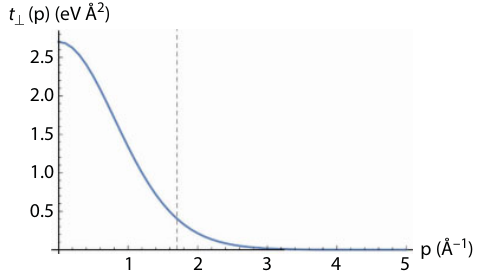
\includegraphics[width=0.6\linewidth]{fig/tperp.png}
\caption{Fourier transform for the interlayer hopping in tBLG. The vertical dashed line marks the position
of the Dirac point. Taken from \cite{handbook2019}.}
\label{fig:tperp}
\end{figure}

%%%%%%%%%%%%%%%%%%%%%%%%%%%%%%%%%%%%%%%%%%%%%%%%%%%%%%%%%%%%%%%%%%%%%%%%%%%%%%%%%%%%%%%%%%%%%%%%%%
\subsection{\textcolor{red}{Small rotation limit}}
%%%%%%%%%%%%%%%%%%%%%%%%%%%%%%%%%%%%%%%%%%%%%%%%%%%%%%%%%%%%%%%%%%%%%%%%%%%%%%%%%%%%%%%%%%%%%%%%%%

When the rotation angle $\theta \lesssim 10^\circ$ is small enough, we can expand around the Dirac points of each layer $\k_\ell = \K_\ell + \q_\ell$ with $\abs{\q_\ell} \sim \abs{\Delta \K} \ll \abs{\K}$. Approximating $t_\perp(\K_1+\q_1+\G_1) \approx t_\perp(\K_1+\G_1)$, the interlayer coupling becomes
$$
T_{12}^{\alpha\beta}(\q_1,\q_2) = \frac{1}{A_{\text{u.c.}}} \sum_{\G_1,\G_2} e^{i\G_1\vdot\vtau_{1,\alpha}}
t_{12}^{\alpha\beta}(\K_1+\G_1) e^{-i\G_2\vdot\vtau_{2,\beta}}
\delta_{\K_1+\q_1+\G_1,\K_2+\q_2+\G_2}.
$$

As $t_\perp(\p)$ decays rapidly with $\abs{\p}$, we truncate $t_\perp(\p) \approx 0$ for $\abs{\p} > \abs{\K}$. This leaves us only three options for $\G_1$, being $\g_{11} = \0$, $\g_{12} = \b_{12}$, $\g_{13} = -\b_{11}$. These three vectors correspond to the three $\K$ equivalent points on the monolayer BZ. Because of the indifference between layer 1 and 2, the same goes for $\G_2$. Notice that $\abs{\K_1+\g_{1n}} = \abs{\K}$, because they are equivalent $\K$ points. Thus, the only quantity that matters is $t_\perp(\abs{\K})$. We have the term
$$
\delta_{\K_1+\q_1+\G_1,\K_2+\q_2+\G_2} = \delta_{\q_2-\q_1,\K_1-\K_2+\G_1-\G_2}.
$$
We call $\Delta\K = \K_1-\K_2$. Due to $\abs{\q_\ell} \ll \abs{\K}$, we only have that $\q_2-\q_1 = \K_1-\K_2+\G_1-\G_2$ if $\G_1 = \g_{1n}$ and $\G_2 = \g_{2n}$ have the same index $n$. Therefore, we have three possibilities
$$
\q_\text{b} = \K_1 - \K_2 = \abs{\Delta \K} \qty(0, -1),
$$
$$
\q_\text{tr} = (\K_1 - \K_2) + (\g_{12} - \g_{22}) = \abs{\Delta \K} \qty(\frac{\sqrt{3}}{2}, \frac{1}{2}),
$$

$$
\q_\text{tl} = (\K_1 - \K_2) + (\g_{13} - \g_{23}) = \abs{\Delta \K} \qty(-\frac{\sqrt{3}}{2}, \frac{1}{2}),
$$
where $\abs{\Delta \K} = 2 \sin(\theta/2) \abs{\K}$.

The interlayer coupling has only three terms
$$
T_{12}^{\alpha\beta}(\q_1,\q_2) =
T^{\alpha\beta}_{\q_\text{b}} \delta_{\q_1-\q_2, \q_\text{b}} +
T^{\alpha\beta}_{\q_\text{tr}} \delta_{\q_1-\q_2, -\q_\text{tr}} +
T^{\alpha\beta}_{\q_\text{tl}} \delta_{\q_1-\q_2, -\q_\text{tl}},
$$
where $T^{\alpha\beta}_{\q_n} = \frac{t_\perp(\abs{\K})}{A_{\text{u.c.}}} e^{i \g_{1n} \vdot \bm{\tau}_{1\alpha}}
e^{-i \g_{2n} \vdot \bm{\tau}_{2\beta}}$. Writing it in the $A, B$ basis we get
$$
T_{\q_\text{b}} = \frac{t_\perp(\abs{\K})}{A_{\text{u.c.}}}
\begin{pmatrix}
1 & 1 \\
1 & 1
\end{pmatrix},
$$
$$
\textcolor{red}{
T_{\q_\text{tr}} = \frac{t_\perp(\abs{\K})}{A_{\text{u.c.}}} e^{-i \g_{12} \vdot \vtau_0}
\begin{pmatrix}
e^{i\phi} & 1 \\
e^{-i\phi} & e^{i\phi}
\end{pmatrix},
}
$$
$$
\textcolor{red}{
T_{\q_\text{tl}} = \frac{t_\perp(\abs{\K})}{A_{\text{u.c.}}} e^{-i \g_{13} \vdot \vtau_0}
\begin{pmatrix}
e^{-i\phi} & 1 \\
e^{i\phi} & e^{-i\phi}
\end{pmatrix},
}
$$
with $\phi = 2\pi/3$.



%%%%%%%%%%%%%%%%%%%%%%%%%%%%%%%%%%%%%%%%%%%%%%%%%%%%%%%%%%%%%%%%%%%%%%%%%%%%%%%%%%%%%%%%%%%%%%%%%%%
%\section{AB stacking}
%%%%%%%%%%%%%%%%%%%%%%%%%%%%%%%%%%%%%%%%%%%%%%%%%%%%%%%%%%%%%%%%%%%%%%%%%%%%%%%%%%%%%%%%%%%%%%%%%%%
%
%The so-called Bernal or AB stacking of two layers of graphene is such that the atoms of sublattice $A$ from one layer are placed above the atoms of sublattice $B$ from the other layer.
%To model the bilayer system in this configuration, we use the monolayer tight-binding hamiltonian (with only the first
%nearest neighbors) as a basis and include an interlayer hopping. Indexing the layers with $\ell = 1, 2$, we write
%\begin{equation} \label{eq:ab-hamil}
%H = H_1 + H_2 + H_{\perp},
%\end{equation}
%\begin{equation} \label{eq:ab-slg-hamil}
%\begin{split}
%H_\ell &= -t \sum_{\R} c_{\ell,A}^\d(\R) [c_{\ell,B}(\R) + c_{\ell,B}(\R-\a_1) + c_{\ell,B}(\R-\a_2)] + \hc, \\
%H_\perp &= t_{\perp} \sum_{\R} c_{1,A}^\d(\R) c_{2,B}(\R) + \hc,
%\end{split}
%%\begin{split}
%%H_1 &= -t \sum_{\R} c_{1,A}^\d(\R) [c_{1,B}(\R) + c_{1,B}(\R-\a_1) + c_{1,B}(\R-\a_2)] + \hc, \\
%%H_2 &= -t \sum_{\R} c_{2,A}^\d(\R) [c_{2,B}(\R) + c_{2,B}(\R-\a_1) + c_{2,B}(\R-\a_2)] + \hc,
%%\end{split}
%\end{equation}
%where $c_{\ell,\alpha}(\R)^\d$ is the creation operator for an electron in a state $\ket{\ell,\R,\alpha}$. Using the discrete Fourier Transform of the creation operators
%\begin{equation} \label{eq:ft-creatio}
%c_{\ell,\alpha}^\d(\R) = \frac{1}{\sqrt{N}} \sum_{\k\in\text{1BZ}} e^{-i\k\vdot(\R+\bm{\tau}_{\ell,\alpha})} c_{\ell,\alpha}^\d(\k),
%\end{equation}
%we can rewrite $H = \sum_{\k} \Psi^\d(\k) H(\k) \Psi(\k)$, where $\Psi^\d(\k) = (c_{1,A}^\d(\k) \; c_{1,B}^\d(\k) \; c_{2,A}^\d(\k) \; c_{2,B}^\d(\k))$ and
%\begin{equation} \label{eq:ab-momentum_space}
%H(\k) =
%\begin{pmatrix}
%0 & -t f(\k) & 0 & t_\perp \\
%-t f^*(\k) & 0 & 0 & 0 \\
%0 & 0 & 0 & -t f(\k) \\
%t_\perp & 0 & -t f^*(\k) & 0 \\
%\end{pmatrix}.
%\end{equation}
%
%Diagonalizing $H(\k)$ we obtain the four bands for the AB-stacked bilayer graphene
%\begin{equation} \label{eq:ab-four_bands}
%E_{\pm,\pm} = \pm t
%\sqrt{
%\qty(\frac{t_\perp}{2t})^2 +
%4 \cos(\frac{\sqrt{3}}{2} d \, k_x) \cos(\frac{3}{2} d \, k_y) + 2 \cos(\sqrt{3} d \, k_x) + 3
%}
%\; \pm \; \frac{t_\perp}{2}.
%\end{equation}






%As drawn in Figure \ref{fig:latvec}, we have
%\begin{align}
%\label{eq:scalarprods0}
%\abs{\a_i^{(j)}} &= a, \\
%\label{eq:scalarprods1}
%\vb{a}_1^{(j)} \vdot \vb{a}_2^{(j)} &= a^2 \cos(60^\circ) = a^2/2, \\
%\label{eq:scalarprods2}
%\vb{a}_1^{(1)} \vdot \vb{a}_1^{(2)} &= a^2 \cos\theta, \\
%\label{eq:scalarprods3}
%\vb{a}_1^{(1)} \vdot \vb{a}_2^{(2)} &= a^2 \cos(60^\circ + \theta), \\
%\label{eq:scalarprods4}
%\vb{a}_1^{(2)} \vdot \vb{a}_2^{(1)} &= a^2 \cos(60^\circ - \theta).
%\end{align}
%
%The superlattice vectors $\vb{L}_1$, $\vb{L}_2$ (when the angle is commensurate) are related by a $60^\circ$ rotation. In general, because $\vb{L}_1$ is a point that belongs to the lattices of both layers, it is written by integers $m,n,m',n'$ as
%\begin{equation} \label{eq:L1}
%\vb{L}_1 = m\vb{a}_1^{(1)} + n\vb{a}_2^{(1)} = m'\vb{a}_1^{(2)} + n'\vb{a}_2^{(2)}.
%\end{equation}
%
%Koshino \cite{koshino2012} argues that there is an appropriate choice of lattice vectors $\vb{a}_1^{(1)}, \vb{a}_2^{(1)}, \vb{a}_1^{(2)}, \vb{a}_2^{(2)}$ (satisfying equations \ref{eq:scalarprods0} to \ref{eq:scalarprods4}) such that the indices $(m',n')$ can be made equal to $(n,m)$. By taking the scalar products of equation \ref{eq:L1} with $\vb{a}_1^{(1)}$ and $\vb{a}_1^{(2)}$, we get
%$$
%\begin{cases}
%\; m + n/2 = n \cos\theta + m \cos(60^\circ + \theta); \\
%\; m/2 + n = m \cos\theta + n \cos(60^\circ - \theta).
%\end{cases}
%\Rightarrow
%\begin{cases}
%\; mn + n^2/2 = n^2 \cos\theta + mn \qty(\frac{\cos\theta}{2}
%- \frac{\sqrt{3} \sin\theta}{2}); \\
%\; m^2/2 + mn = m^2 \cos\theta + mn \qty(\frac{\cos\theta}{2}
%+ \frac{\sqrt{3} \sin\theta}{2}).
%\end{cases}
%$$
%
%Summing the two equations above gives us
%\begin{equation} \label{eq:costheta}
%\boxed{\cos\theta = \frac{1}{2} \cdot \frac{m^2 + n^2 + 4mn}{m^2 + n^2 + mn}.}
%\end{equation}



%\n
%
%\textbf{TEXTO ABAIXO FOI PLAGIADO DO ZOU2018}
%
%Theoretically at small twist angles, there is a well
%known “continuum theory” description which yields
%well-defined band structures for all twist angles in-
%cluding incommensurate ones [32, 33].
%The contin-
%uum theory reveals many universal features of the band
%structure, such as the existence of Dirac crossings be-
%tween valence and conduction bands within each val-
%ley of the underlying graphene layers. These features
%have been benchmarked against tight-binding calcula-
%tions on commensurate structures [34–37]. They are
%also nicely consistent with experiments at twist angles
%larger than the magic angles (where correlation effects
%are expected to be weaker, and band theory predic-
%tions can be reasonably compared with experiment).
%In particular, Cao et al showed that at a twist angle of
%about 1.8 degrees the Landau fan structure near charge
%neutrality is exactly what is expected from the Dirac
%points predicted by the continuum theory [38]. Despite
%its success for qualitative universal aspects, quantita-
%tively the continuum theory yields a very small value
%compared to experiments for the gap separating the
%nearly flat bands from other bands. This discrepancy is
%believed to be reduced once effects of lattice relaxation
%and electron interactions are included. Formally these
%additional effects can be included phenomenologically
%in the continuum model by modifying its parameters
%away from those estimated microscopically [6, 21].
%Apart from translational symmetry, the approxima-
%tions involved in the continuum theory build in a num-
%ber of other point group symmetries which are not fully
%present in any commensurate structure. These include
%a C6 rotation symmetry, and a valley Uv(1) associated
%with separate conservation of electrons associated with
%each valley.
%This symmetry structure of the contin-
%uum theory is essential in protecting the Dirac points
%of valley filtered bands. Specifically, on top of the val-
%ley Uv(1) (needed to define separate bands within each
%valley) a C2T = C3
%6T symmetry is able to protect the
%Dirac points from acquiring a gap.
%Even restricting
%to commensurate structures with translation symme-
%try, Uv(1), and maybe even C2T , are not both exact
%microscopic symmetries.
%
%In the older literature it was appreciated that at
%small twist angles the extra symmetries of the contin-
%uum theory are excellent approximations [34–36, 39].
%Furthermore it was understood that there is essentially
%no difference between incommensurate and commen-
%surate structures, or between distinct commensurate
%structures with different exact microscopic symmetries.
%These issues have re-emerged in recent discussions of
%TBG, and have led to some confusion. We therefore
%carefully review and collect together some pertinent
%facts about different commensurate structures, their
%relationship to the continuum theory, and the implica-
%tions for a description of small angle (possibly incom-
%mensurate) TBG.
%
%The most fundamental aspect of our previous dis-
%cussion of the band structure is the existence of an ob-
%struction to constructing well localized Wannier func-
%tions transforming naturally under all symmetry oper-
%ations. The obstruction relies strongly on the presence
%of symmetries that are not exact microscopic symme-
%tries.
%Why then should we worry about it?
%Let us
%therefore review the tight logic that forces us to con-
%front it. As reviewed above, it is a robust feature of
%both theory and experiment that to excellent accuracy
%there is a good valley Uv(1) symmetry and that within
%each valley there are Dirac band crossings (down to en-
%ergy scales currently accessible in experiments). The
%robustness of the Dirac crossings within each valley
%suggests that it is a symmetry protected feature of the
%band structure. The natural protecting symmetry then
%is C2T as is seen explicitly in the continuum theory.
%For a general small-angle, incommensurate TBG struc-
%ture, the C2 symmetry—like translations itself—is not
%an exact symmetry, but it must be excellent enough
%to give the Dirac cones. This then forces us to study
%systems which have translations, valley Uv(1), and C6
%as good symmetries. However the implementation of
%all these symmetries in the band structure leads to a
%Wannier obstruction.




%%%%%%%%%%%%%%%%%%%%%%%%%%%%%%%%%%%%%%%%%%%%%%%%%%%%%%%%%%%%%%%%%%%%%%%%%%%%%%%%%%%%%%%%%%%%%%%%%%
%%%%%%%%%%%%%%%%%%%%%%%%%%%%%%%%%%%%%%%%%%%%%%%%%%%%%%%%%%%%%%%%%%%%%%%%%%%%%%%%%%%%%%%%%%%%%%%%%%


%%%%%%%%%%%%%%%%%%%%%%%%%%%%%%%%% COMMENT THIS TO COMPILE main.tex %%%%%%%%%%%%%%%%%%%%%%%%%%%%%%%%
%%%-----
%%% Referências bibliográficas
%%%-----
%\addcontentsline{toc}{chapter}{\bibname}
%%\bibliographystyle{abntex2-num}
%\bibliography{citations}
%\bibliographystyle{ieeetr}
%\end{document}
%%%%%%%%%%%%%%%%%%%%%%%%%%%%%%%%% COMMENT THIS TO COMPILE main.tex %%%%%%%%%%%%%%%%%%%%%%%%%%%%%%%%
